\chapter{Preliminary work}\label{chap:preliminary-work}

\section*{}

This chapter will present some preliminary work that was developed for the \gls{clarissa} European research project\footnote{\url{http://www.smerobotics.org/AUTOMATICA/exhibit-07-2016.html}}. It will give an overview of two projection mapping prototypes that were designed for cooperative welding between a dual arm robot and a human operator. The main goal of these prototypes is to increase the operator productivity while also improving the quality of their work by projecting both the sequence and the welding place of objects (avoiding manual / inaccurate measuring of the welding objects places). The first prototype\footnote{\url{https://github.com/inesc-tec-robotics/gazebo_projection_mapping}} was developed for \gls{dlp} projectors and extended the Gazebo simulator\footnote{\url{http://gazebosim.org}} functionality to allow the generation of raster images from the \gls{cad} models with the proper perspective view and lens distortion in order to achieve sub-millimeter accuracy of the projection information. The second prototype\footnote{\url{https://github.com/carlosmccosta/eyeshot_projection_mapping}} was implemented using devDept Eyeshot rendering engine\footnote{\url{https://www.devdept.com}} for galvanometer scanners, given that they allow to project information with high accuracy in three-dimensional objects without losing image focus and also have very good brightness, which is required for most industrial applications in which the workspace is highly illuminated.


\section{Methodology}

The first prototype was developed for \gls{dlp} projectors given their higher availability, consistent image refresh rate and also lower cost. The first step was to attach a \gls{dlp} projector in a stable platform and in a position that allowed to project information in all the intended workplace while trying to minimize projection occlusions and ensuring image focus. The second step relied on computer vision algorithms to retrieve the intrinsic parameters of the projector, such as the x and y focal lengths, projection principal point and lens distortion coefficients along with the extrinsic parameters, such as the 3D position and rotation of the projector in the global workspace coordinate system. These calibration parameters allowed to model the projector within the Gazebo simulator in order to be able to generate raster images of the welding information / \gls{cad} models with the proper perspective view while also reducing the projection error caused by the projector lens distortion.

The second prototype followed a similar methodology, but unlike the \gls{dlp} projector that required a simple manual adjustment of the lens focus, galvanometer scanners rely on two moving mirrors that need to be manually fine-tuned with ten potentiometers in order to reduce overshoots and undershoots using high / low frequency damping and servo gain adjustments while also ensuring proper scaling and projection center. Later on, the calibration parameters were computed using computer vision methods and the projector was modeled within Eyeshot in order to generate vector images of the welding information / \gls{cad} models with the proper perspective view while also reducing laser projection distortion.


\section{Projector modeling}

Over the years, several projection technologies were developed according to the requirements of color fidelity / saturation, image sharpness, brightness, contrast, refresh rate and price. Currently, the video projection market is split between reflective \gls{dlp} and transmissive \gls{lcd} projection technology, with a small percentage of projectors consisting of a hybrid between the two technologies (\gls{lcos}).

For video projection mapping purposes \cite{Bimber2005,Fujimoto2014,Raskar1998,Tan2013}, reflective projectors are better suited than the remaining technologies given their ability to create images with smaller gaps between the projected pixels (smoother images) and they also have higher contrast, better color accuracy / uniformity, much fewer dead pixels and the image quality does not degrade over time. The main stages of the image creation in a \gls{dlp} projector are show in \cref{fig:dlp-projector-diagram-1-dmd}. The first phase is the generation of light from either a lamp or a \gls{led} / laser array, which is later on condensed on a lens in order to pass through a moving color wheel to become one of the 3 primary additive colors (red, green, blue). The colored light then passes through a shaping lens and hits a \gls{dmd} which has an electronic controllable mirror for each projection pixel that either reflects the light into the projection lens or into a heat sink. Color shading is achieved by controlling how long and how often the micro mirrors in the \gls{dmd} are reflecting each light color into the lens (or into the heat sink).

For industrial applications of projection mapping in which the goal is to project \gls{cad} drawings, galvanometers scanners using a single laser offer higher precision and brightness than video projectors, at the cost of much lower image refresh rate and much higher price. The images are generated by aiming the laser light using two mirrors moving at very high speeds (example of laser reflection shown in \cref{fig:laser-projector-diagram-1-colors}).


\begin{figure}[H]
	\begin{floatrow}[2]
		\ffigbox[\FBwidth]
		{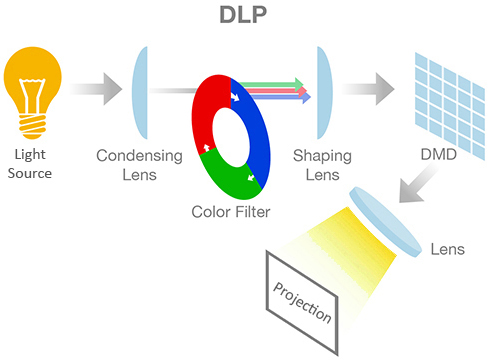
\includegraphics[height=.22\textheight]{preliminary-work/dlp-projector-diagram-1-dmd}}
		{\caption[Single chip \glsentrytext{dlp} diagram]{Single chip \glsentrytext{dlp} diagram\protect\footnotemark}\label{fig:dlp-projector-diagram-1-dmd}}
		\ffigbox[\FBwidth]
		{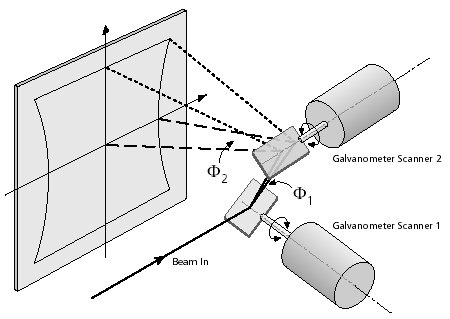
\includegraphics[height=.22\textheight]{preliminary-work/laser-projector-diagram-1-colors}}
		{\caption[Single laser galvanometer scanner diagram]{Single laser galvanometer scanner diagram\protect\footnotemark}\label{fig:laser-projector-diagram-1-colors}}
	\end{floatrow}
\end{figure}
\footnotetext[\the\numexpr\value{footnote}-1\relax]{\url{https://vimeo.com/blog/post/display-tech-home-projectors}}
\footnotetext[\value{footnote}]{\url{http://www.zamisel.com/SSpostavka2.html}}


The mathematical modeling of a \gls{dlp} projector can be seen as an inverse camera, given the grid disposition of the mirrors in the \gls{dmd} and the usage of a lens to focus the light into the projection surface. The galvanometer scanners model is slightly different since there is no lens and no focal point, but it can be approximated by a pinhole camera for efficient scene rendering using \gls{opengl} / Direct3D, with later distortion correction using the mathematical models proposed in \cite{Manakov2011}.

Both projection mapping prototypes modeled the projector with a pinhole camera \cite{Hartley2003} (shown in \cref{fig:camera-intrinsics}) using the \gls{opengl} / Direct3D projection matrix. The matrix formulation for computing the projection matrix is shown in \cref{eq:projection-matrix,eq:ndc-matrix,eq:perspective-matrix}, and it includes the focal lengths (Fx, Fy), principal point (Cx, Cy) and axis skew (S) intrinsic parameters (in pixel units). The correction of lens distortion for \gls{dlp} projectors used 3 coefficients for removing radial distortions and 2 coefficients for accounting for the tangential distortions. The correction of the galvanometer scanners distortion (seen in \cref{fig:laser-projector-diagram-1-colors}) is performed by warping the projection points using the MediaLas LaserCAM application in order to remove the distortion that occurs mainly in the horizontal axis.


\begin{equation}\label{eq:projection-matrix}
	ProjectionMatrix = \glsentrytext{ndc}Matrix \times PerspectiveMatrix
\end{equation}

\begin{equation}\label{eq:ndc-matrix}
	NDCMatrix = 
	\begin{bmatrix}
		\frac{2}{ImageWidth} & 0 & 0 & -1 \\
		0 & \frac{2}{ImageHeight} & 0 & -1 \\
		0 & 0 & \frac{-2}{ClipFar - ClipNear} & \frac{-(ClipFar + ClipNear)}{ClipFar - ClipNear} \\
		0 & 0 & 0 & 1
	\end{bmatrix}
\end{equation}


\begin{equation}\label{eq:perspective-matrix}
	PerspectiveMatrix = 
	\begin{bmatrix}
		Fx & S & -Cx & 0 \\
		0 & Fy & -Cy & 0 \\
		0 & 0 & ClipNear + ClipFar & ClipNear \times ClipFar \\
		0 & 0 & -1 & 0
	\end{bmatrix}
\end{equation}


\begin{figure}[H]
	\centering
	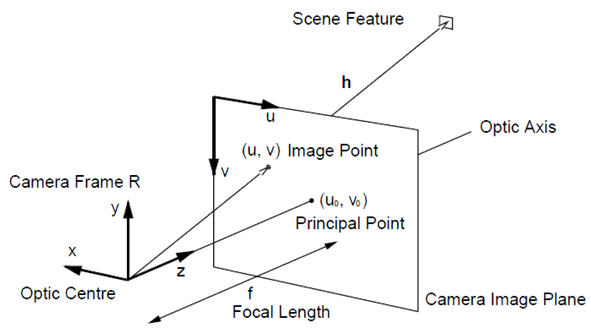
\includegraphics[width=0.7\linewidth]{preliminary-work/camera-intrinsics}
	\caption[Pinhole camera model]{Pinhole camera model\protect\footnotemark}
	\label{fig:camera-intrinsics}
\end{figure}
\footnotetext{\url{http://perso.ensta-paristech.fr/~filliat/Courses/2011_projets_C10-2/BRUNEAU_DUBRAY_MURGUET/monoSLAM_bruneau_dubray_murguet_en.html}}


\section{Projector calibration}

High accuracy projection requires proper hardware / software calibration of the projectors and also appropriate positioning within the intended workspace in order to avoid occlusions caused by the objects 3D shape or the human operators. The next sections will detail the required calibration steps for both \gls{dlp} projectors and galvanometer scanners.


\subsection{\glsentrytext{dlp} projector calibration}

The intrinsic parameters of a \gls{dlp} projector can be computed using image analysis of complementary gray code patterns (seen in \cref{fig:dlp-calibration-pattern-wall}) projected into a chessboard. The calibration system proposed in \cite{Moreno2012} was used to retrieve the 5 intrinsic parameters (Fx, Fy, Cx, Cy, S) of the projector along with the 3D position and rotation of the projector in relation to the camera. It was used 5 sets of 42 gray code image patterns captured with the chessboard in different positions and orientations in relation to the projector, that was at a distance of 2.2 meters from the table workspace. After calibration it was projected a validation pattern to evaluate the accuracy of the projection, and it can be seen in \cref{fig:dlp-projected-chessboard} that the white squares were projected into the chessboard with sub-millimeter accuracy.


\begin{figure}[H]
	\begin{floatrow}[2]
		\ffigbox[\FBwidth]
		{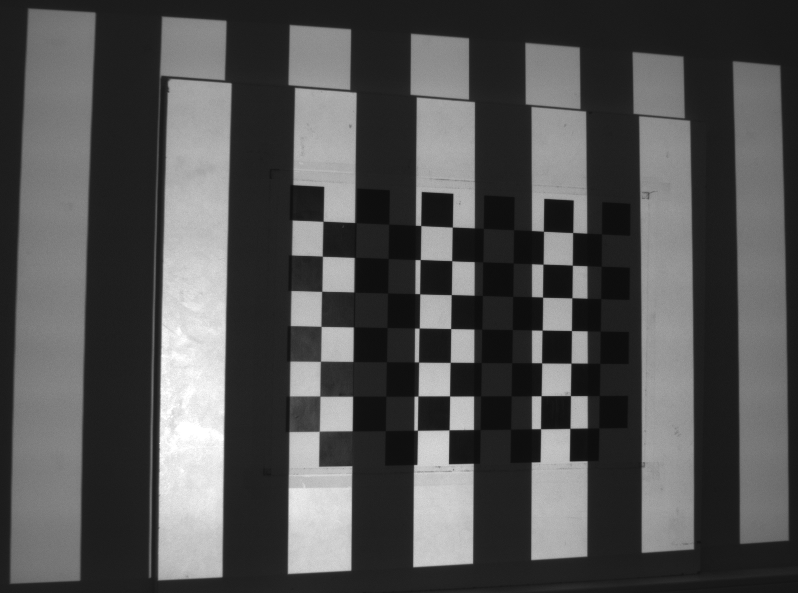
\includegraphics[height=.217\textheight]{preliminary-work/dlp-calibration-pattern-wall}}
		{\caption{One of the \glsentrytext{dlp} projector calibration patterns}\label{fig:dlp-calibration-pattern-wall}}
		\ffigbox[\FBwidth]
		{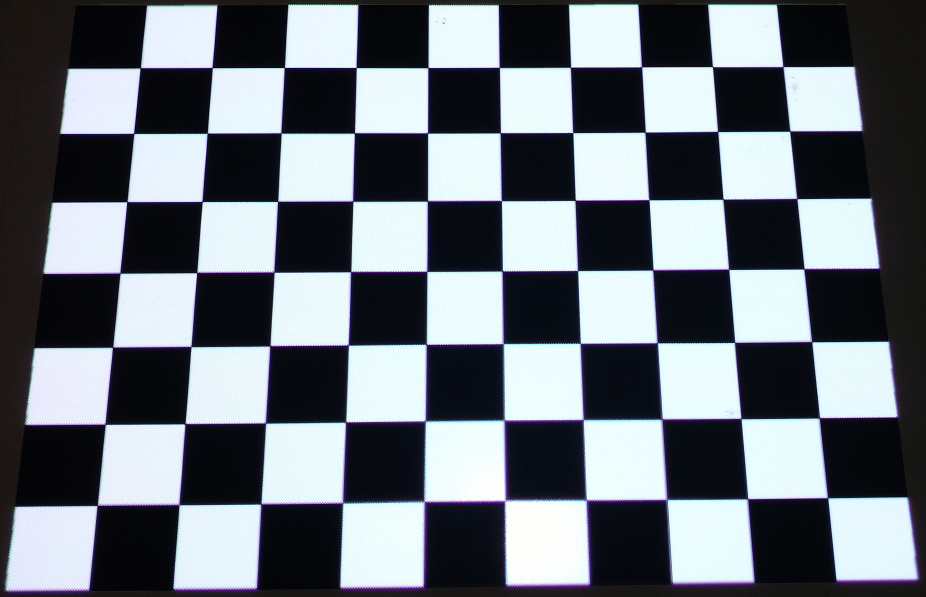
\includegraphics[height=.217\textheight]{preliminary-work/dlp-projected-chessboard}}
		{\caption{\glsentrytext{dlp} projector validation pattern}\label{fig:dlp-projected-chessboard}}
	\end{floatrow}
\end{figure}


\subsection{Galvanometer scanner calibration}

Analog galvanometer scanners controlled with \gls{pid} controllers require manual fine tuning of the x and y galvos\footnote{\url{http://www.medialas-industrial.de/ctigalvos.html?&L=1}} in order to achieve high projection accuracy. The MediaLas ILP 622 projector\footnote{\url{http://www.medialas-industrial.de/ilp622-laserprojektor.html?&L=1}} used is equipped with two MicroAmp\footnote{\url{http://www.medialas-industrial.de/microamp.html?&L=1}} drivers (one for each galvo), that allow manual calibration using 5 potentiometers. One of the potentiometers can be used to adjust the maximum field of view of a galvo, which is useful to ensure that the galvanometer scanner is projecting squares as squares and not as rectangles. Another potentiometer is for adjusting the center of projection, which can help to reduce small errors in the mounting of the galvos within the projector frame. The last 3 potentiometers are for reducing undershoots and overshoots of the laser projection, using high and low frequency damping and adjustable servo gain. The standard procedure for calibrating galvanometers scanners uses the \gls{ilda} test pattern at 30000 \gls{pps} with a deflection angle of the galvos at 8º (shown in \cref{fig:laser-ilda-calibration-pattern}). A properly calibrated galvanometer scanner (example in \cref{fig:laser-ilda-calibration-pattern-projected}) projecting perpendicularly at 2 meters from this pattern will have the large circle with the same diameter as the small inner square edges and will also have a correct center of projection, proper laser blanking and straight lines forming an outer square with 28 centimeter edges.

Galvanometer scanners have adjustable galvo moving speed which can be increased in order to reduce image flickering (at the cost of projection deformation) or reduced to ensure high accuracy projection. This is an important calibration parameter that must be tuned as a trade-off between projection accuracy and image stability.

The MediaLas ILP 622 draws points / lines within a canvas of 32-bit range, but in order to be able to model the projector within Eyeshot Direct3D rendering engine it was created a drawing area of $2000 \times 2000$ units to generate the scene images. Later on, the vector image points were scaled to match the 32-bit projection canvas. The camera x and y focal lengths (in pixels) were computed in relation to this $2000 \times 2000$ drawing area by measuring the maximum projection area of the projector at 2 meters and using the mathematical formulas shown in \cref{eq:intrinsics-focal-lenghts,eq:intrinsics-field-of-view}. The principal point was calibrated using the galvo driver’s potentiometers and the sensor axis skew was negligible in the MediaLas ILP 622.

The galvanometer scanner calibration achieved sub-millimeter accuracy, as can be seen by analyzing the validation pattern shown in \cref{fig:laser-calibration-validation}. Only the bottom part of the chessboard was projected in order to reduce image flickering (given that the galvos moving speed was reduced to avoid laser projection deformations).

\begin{figure}[H]
	\begin{floatrow}[2]
		\ffigbox[\FBwidth]
		{
\includegraphics[height=.25\textheight]{preliminary-work/laser-ilda-calibration-pattern}}
		{\caption{\glsentrytext{ilda} calibration pattern}\label{fig:laser-ilda-calibration-pattern}}
		\ffigbox[\FBwidth]
		{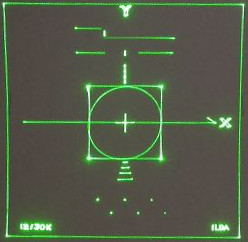
\includegraphics[height=.25\textheight]{preliminary-work/laser-ilda-calibration-pattern-projected}}
		{\caption[Projection of the \glsentrytext{ilda} calibration pattern]{Projection of the \glsentrytext{ilda} calibration pattern\protect\footnotemark}\label{fig:laser-ilda-calibration-pattern-projected}}
	\end{floatrow}
\end{figure}
\footnotetext{\url{http://elm-chan.org/works/vlp/report_e.html}}

\begin{equation}\label{eq:intrinsics-focal-lenghts}
	Fx = \frac{\scriptstyle ImageWidth}{2 \times \tan \frac{HorizontalFieldOfView}{2}},
	Fy = \frac{\scriptstyle ImageHeight}{2 \times \tan \frac{VerticalFieldOfView}{2}}
\end{equation}

\begin{equation}\label{eq:intrinsics-field-of-view}
	HFOV = 2 \times \tanh \frac{\frac{MaxProjectionWidth}{2}}{\scriptstyle ProjectorDistanceToWall},
	HFOV = 2 \times \tanh \frac{\frac{MaxProjectionHeight}{2}}{\scriptstyle ProjectorDistanceToWall}
\end{equation}

\begin{figure}[H]
	\centering
	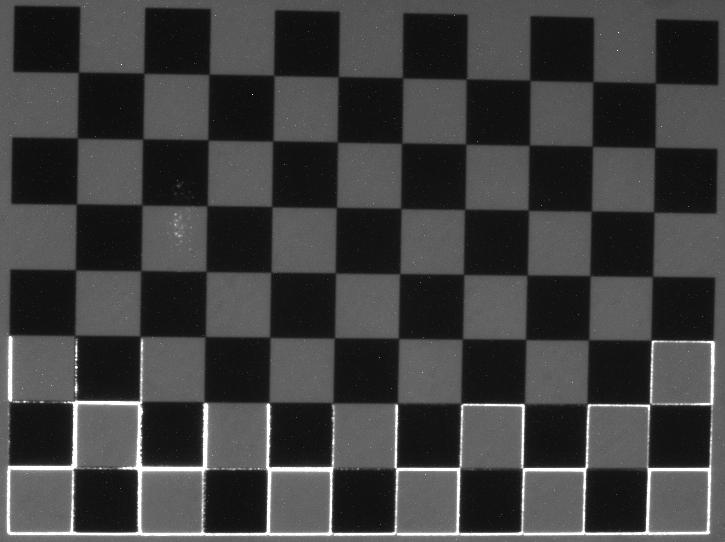
\includegraphics[width=0.49\linewidth]{preliminary-work/laser-calibration-validation}
	\caption{Galvanometer scanner validation pattern}
	\label{fig:laser-calibration-validation}
\end{figure}


\subsection{Camera extrinsics calibration}

For fast recalibration of the projector 3D position and orientation in the global coordinate system of the workspace, both the \gls{dlp} projector and galvanometer scanner had a 5 \gls{mp} Mako G-503B\footnote{\url{https://www.alliedvision.com/en/products/cameras/detail/Mako\%20G/G-503.html}} camera firmly attached to the projectors support. As such, the global position of the projector is given by multiplying the $4 \times 4$ homogeneous matrix that gives the transformation from the chessboard corner (shown in \cref{fig:chess-board-detection}) to the camera, with the $4 \times 4$ homogeneous matrix that gives the transformation from the camera to the projector.

For the \gls{dlp} projector the camera-to-projector matrix was computed using the software described in \cite{Moreno2012}. For the galvanometer scanner this matrix was calculated by placing the projector at 2 meters from a wall, properly leveled in order to ensure that the laser beam was hitting the wall perpendicularly, and then placing a chessboard in the wall in such a way that the center of projection was hitting one of the chessboard corners. By knowing the projector and camera position / orientation in relation to a known coordinate system (the chessboard origin), the transformation from the camera to the galvanometer scanner can be easily computed using \cref{eq:extrinsics-camera-projector}.

\begin{small}
	\begin{equation}\label{eq:extrinsics-camera-projector}
		CameraToProjectorMatrix = ProjectorToChessboardOrigin \times (CameraToChessboardOrigin^{-1})
	\end{equation}
\end{small}

\begin{figure}[H]
	\centering
	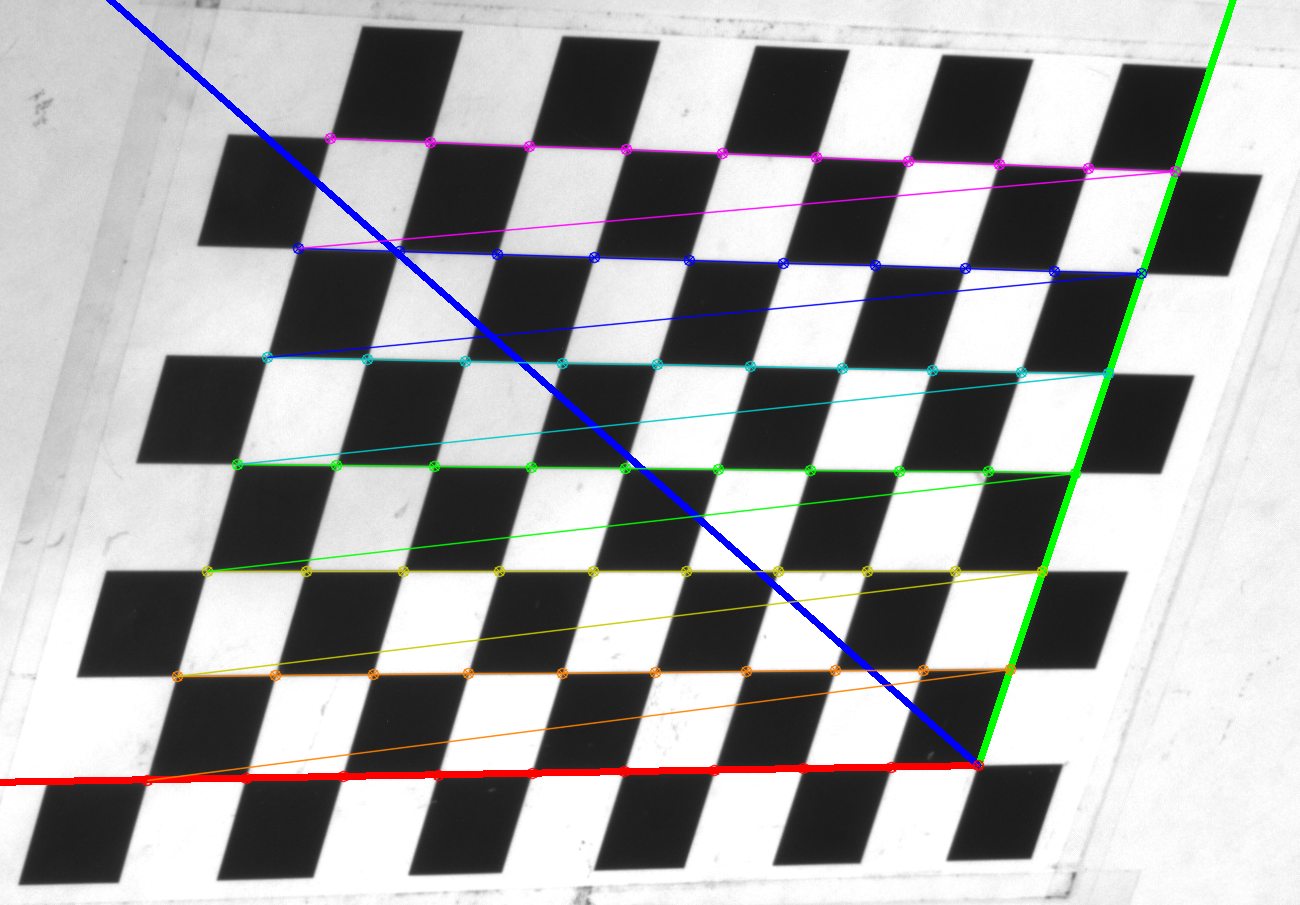
\includegraphics[width=0.59\linewidth]{preliminary-work/chess-board-detection}
	\caption{Example of chessboard origin detection}
	\label{fig:chess-board-detection}
\end{figure}



\section{Scene rendering}

For efficient scene rendering, both projection mapping prototypes relied on \gls{gpu} \glspl{api} to take advantage of the massively parallel graphics cards currently available. The Gazebo simulator relied on the cross platform open source Ogre3D graphics engine\footnote{\url{http://www.ogre3d.org}} to generate raster images for the \gls{dlp} projectors (example in \cref{fig:dlp-projection-image}), while Eyeshot used the Microsoft proprietary Direct3D rendering engine, which supports native rendering of vector graphics scenes (useful for generating vector images from \gls{cad} models and vector drawings which are required when using galvanometer scanners).

For user interface, the Gazebo simulator allows visual inspection of the scene (shown in \cref{fig:gazebo-user-interface}) while also giving the option to add new objects or move and rotate existing models. The Eyeshot prototype also allows to inspect the scene and has a dedicated interface for validating and adjusting the projector intrinsic and extrinsic parameters (seen in \cref{fig:eyeshot-user-interface-vector-lines}).

\begin{figure}[H]
	\begin{floatrow}[2]
		\ffigbox[\FBwidth]
		{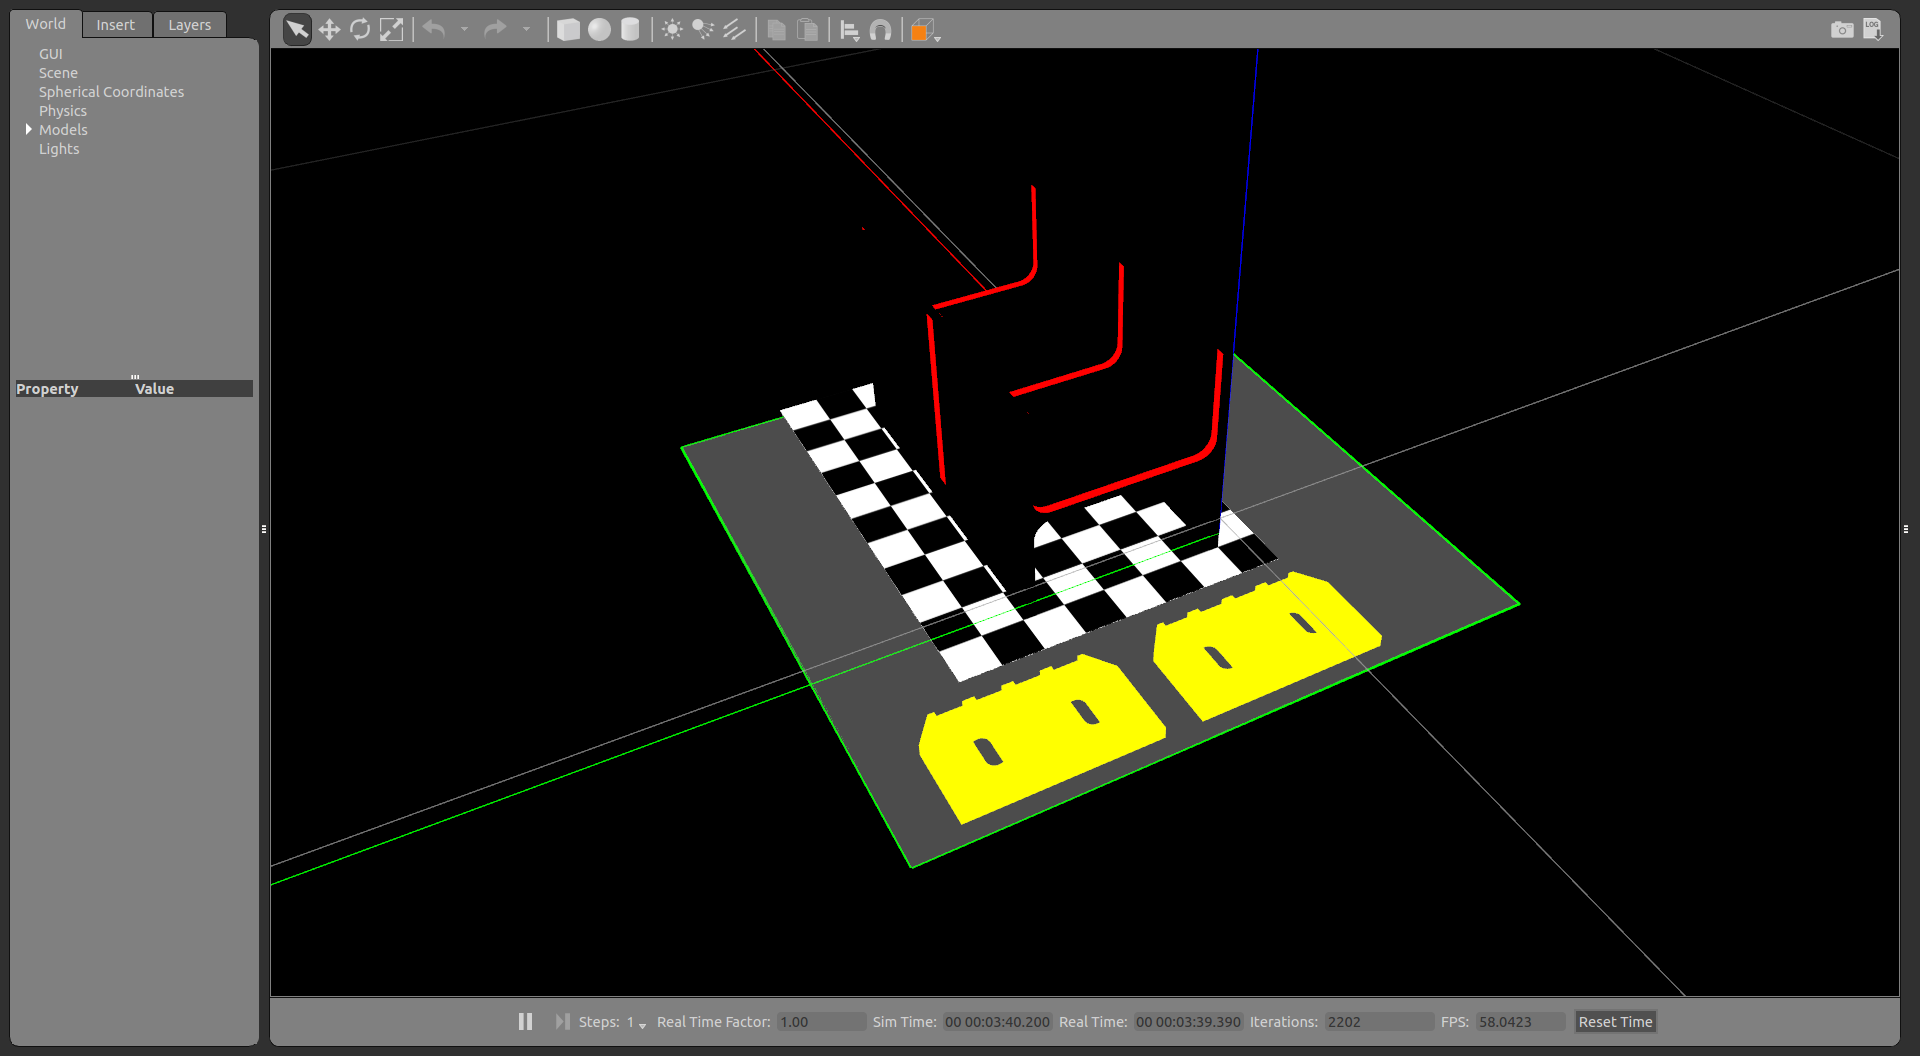
\includegraphics[height=.175\textheight]{preliminary-work/gazebo-user-interface}}
		{\caption{Gazebo user interface}\label{fig:gazebo-user-interface}}
		\ffigbox[\FBwidth]
		{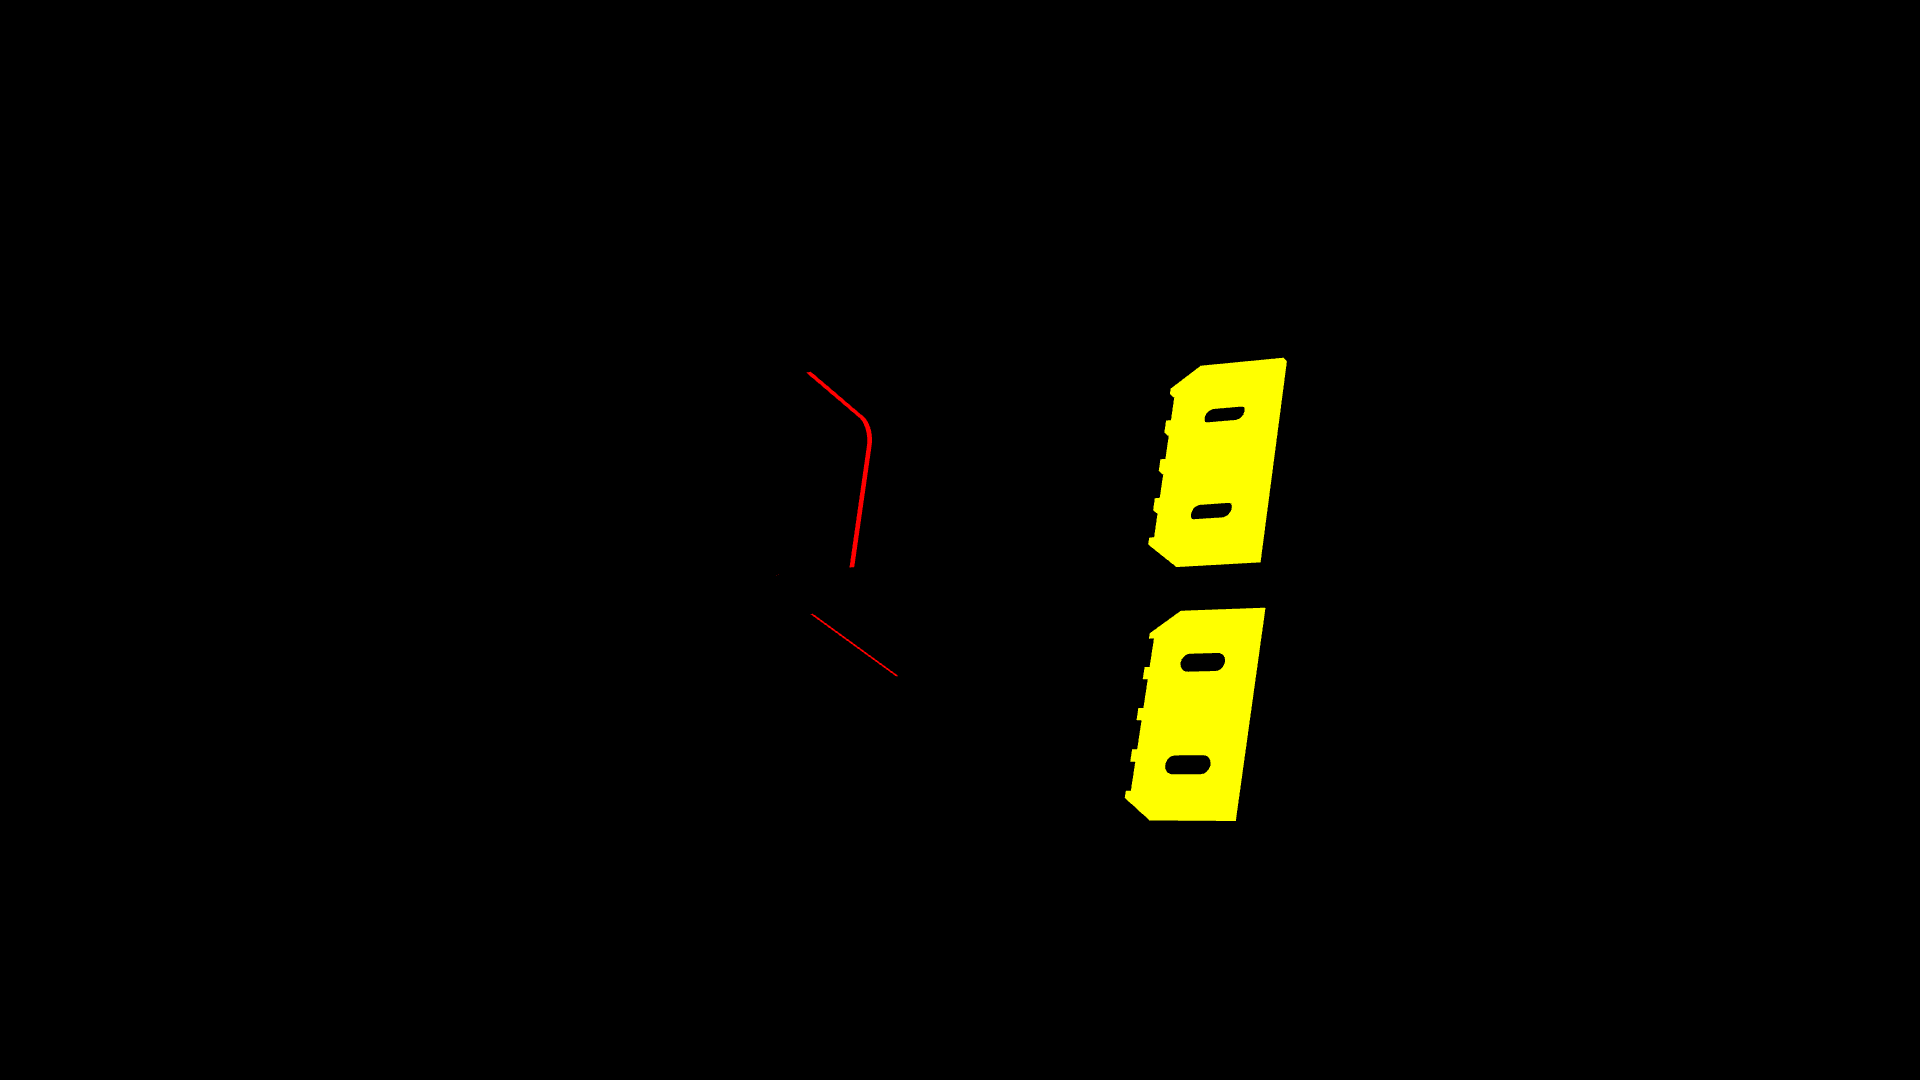
\includegraphics[height=.175\textheight]{preliminary-work/dlp-projection-image}}
		{\caption{Gazebo raster rendering}\label{fig:dlp-projection-image}}
	\end{floatrow}
\end{figure}

\begin{figure}[H]
	\centering
	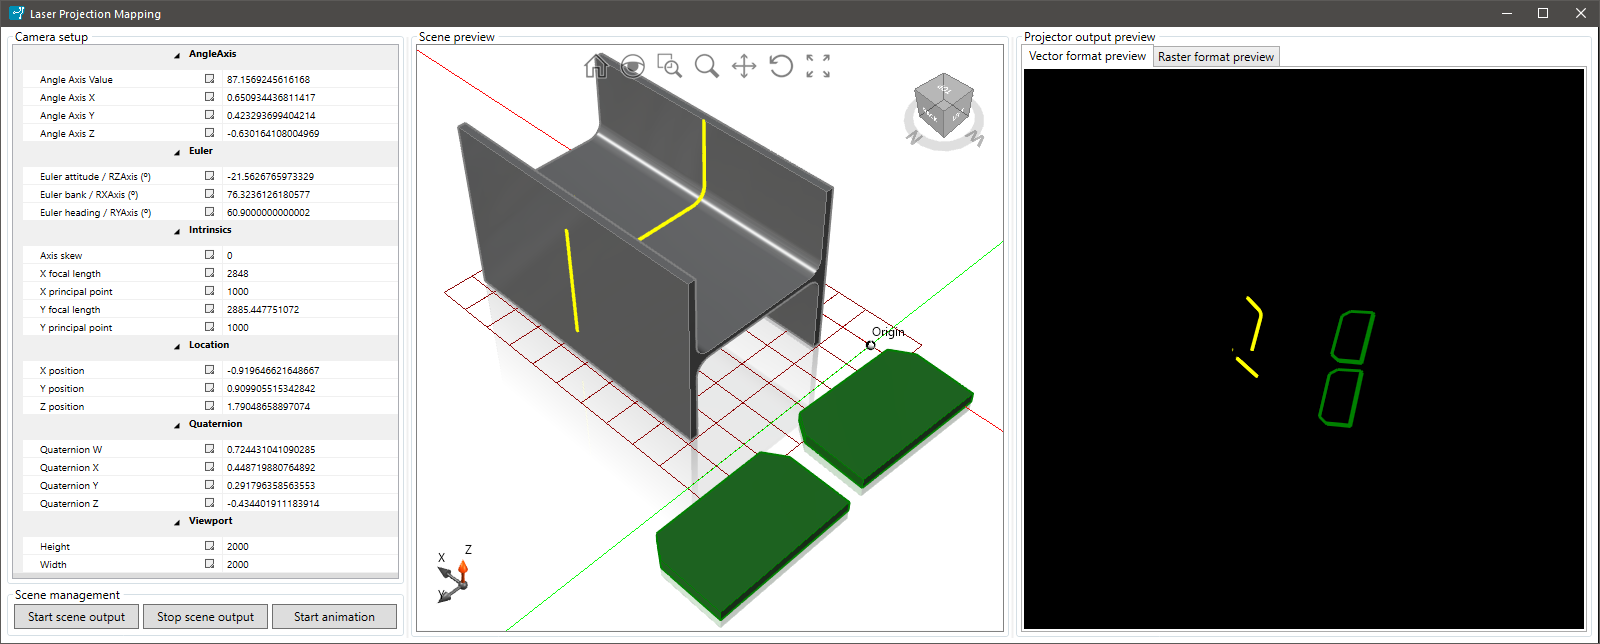
\includegraphics[width=\linewidth]{preliminary-work/eyeshot-user-interface-vector-10px-lines}
	\caption{Eyeshot user interface with scene preview and vector / raster rendering}
	\label{fig:eyeshot-user-interface-vector-lines}
\end{figure}



\section{Projection demonstrations}

Several projection demonstrations were performed over the course of the prototypes development, both in laboratorial and industrial conditions using either \gls{dlp} projectors or the MediaLas ILP 622 galvanometer scanner.


\subsection{\glsentrytext{dlp} projectors demonstrations}

In \cref{fig:dlp-welding-place,fig:dlp-side-projection} it can be seen three-dimensional projection of welding information into a beam using an Acer K132+ \gls{dlp} projector\footnote{\url{http://www.david-3d.com/en/products/accessories/acer_k132_plus}} in laboratorial conditions within a controlled lighting environment, while in \cref{fig:dlp-welding-place-middle-and-side-red,fig:dlp-welding-place-with-object} it can be observed a similar demonstration in industrial conditions within a highly illuminated environment using a BenQ W1070 \gls{dlp} projector\footnote{\url{http://www.benq.com/product/projector/w1070}}. Analyzing these figures, it can be perceived that the projection had sub-millimeter accuracy and that its visibility was dependent on the environment lighting conditions, projected colors, thickness of the projection information and also angle of the projected light into the environment surfaces.

\begin{figure}[H]
	\begin{floatrow}[2]
		\ffigbox[\FBwidth]
		{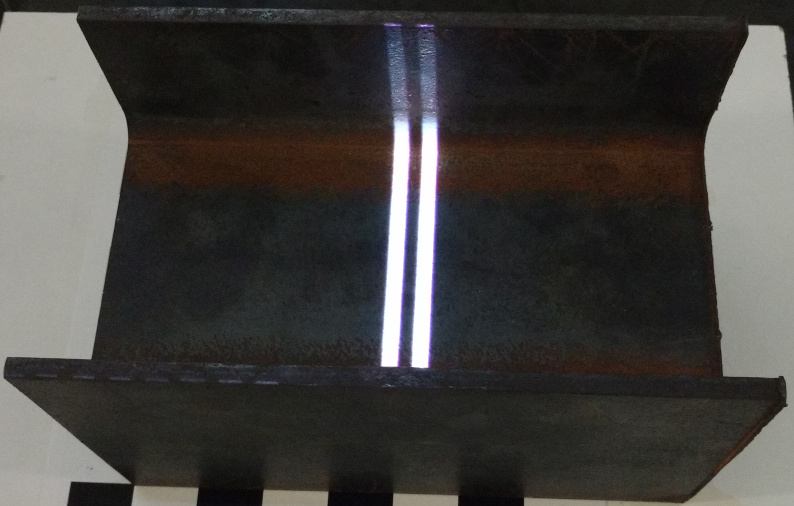
\includegraphics[height=.2\textheight]{preliminary-work/dlp-welding-place}}
		{\caption{Welding projection in middle of beam}\label{fig:dlp-welding-place}}
		\ffigbox[\FBwidth]
		{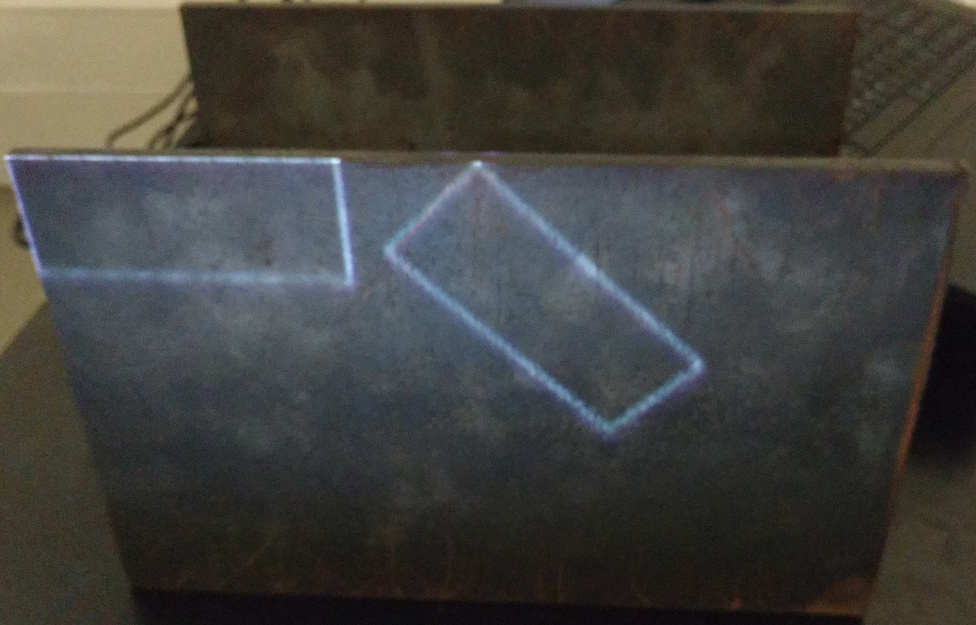
\includegraphics[height=.2\textheight]{preliminary-work/dlp-side-projection}}
		{\caption{Welding projection on side of beam}\label{fig:dlp-side-projection}}
	\end{floatrow}
\end{figure}

\begin{figure}[H]
	\begin{floatrow}[2]
		\ffigbox[\FBwidth]
		{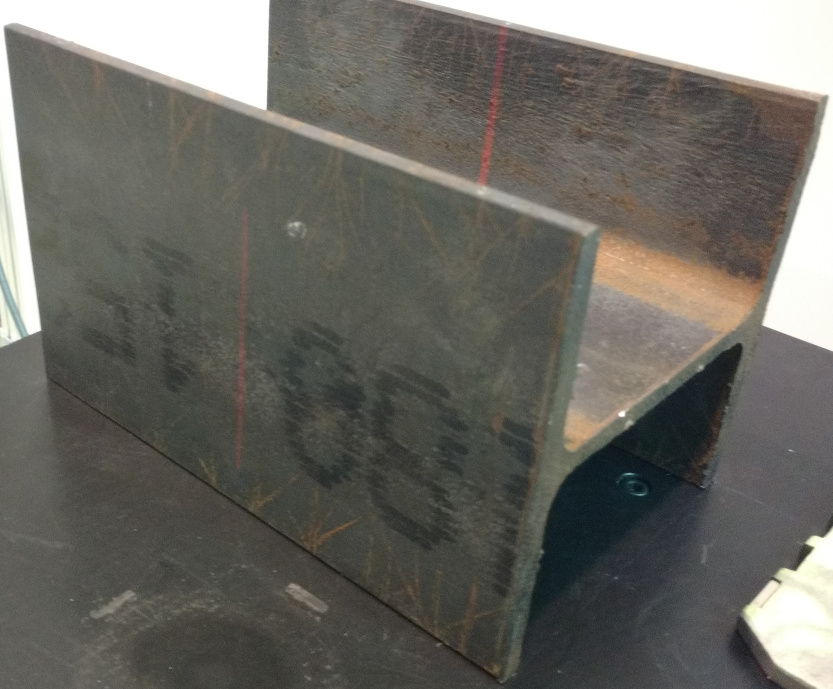
\includegraphics[height=.225\textheight]{preliminary-work/dlp-welding-place-middle-and-side-red}}
		{\caption{Welding projection on middle and side of beam}\label{fig:dlp-welding-place-middle-and-side-red}}
		\ffigbox[\FBwidth]
		{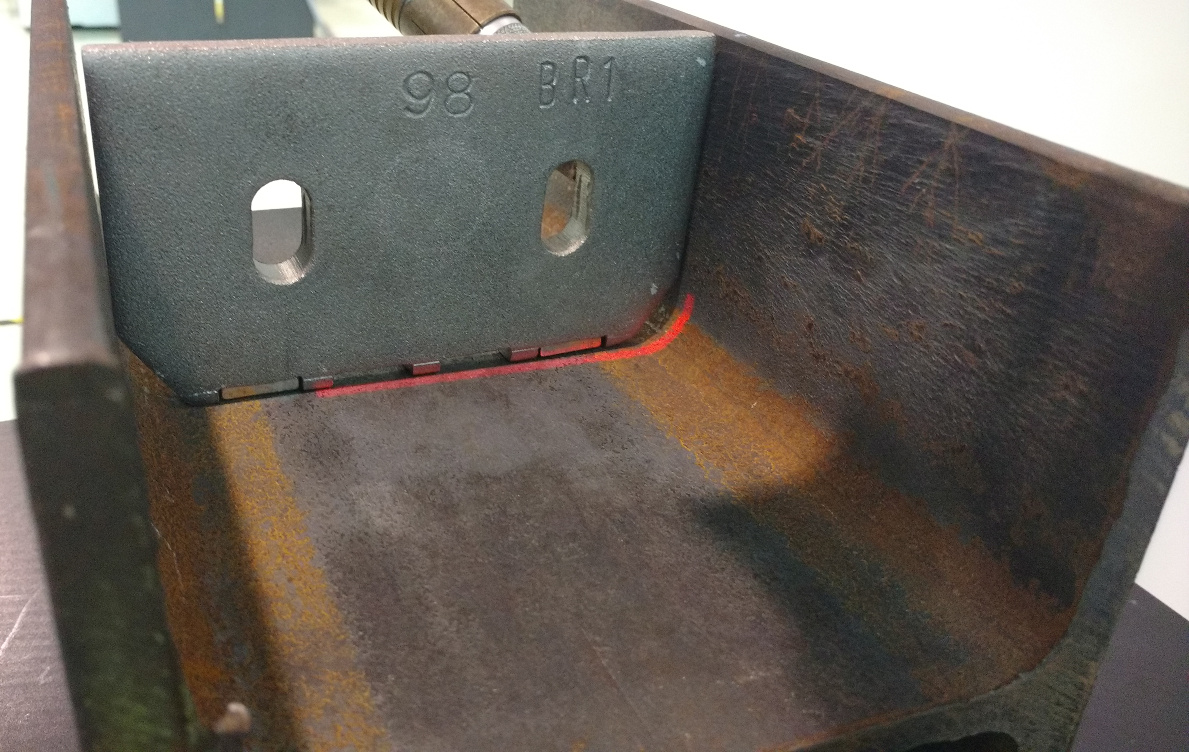
\includegraphics[height=.225\textheight]{preliminary-work/dlp-welding-place-with-object}}
		{\caption{Welding projection on middle of beam}\label{fig:dlp-welding-place-with-object}}
	\end{floatrow}
\end{figure}


\subsection{Galvanometer scanner demonstrations}

In \cref{fig:laser-beam-outline-with-chessboard-and-welding,fig:laser-beam-outline-with-welding} it is shown the projection of three-dimensional information into a beam using the MediaLas ILP 622 galvanometer scanner in laboratorial conditions in a highly illuminated environment. \Cref{fig:laser-object-outline,fig:laser-welding-place} shows a similar demonstration in industrial conditions with only ambient light in which the object outline and the welding place was projected. Analyzing the beam and object outlines and also the projected chessboard, it can be observed that the projection had sub-millimeter accuracy and it is visible in a wide range of lighting conditions.

\begin{figure}[H]
	\begin{floatrow}[2]
		\ffigbox[\FBwidth]
		{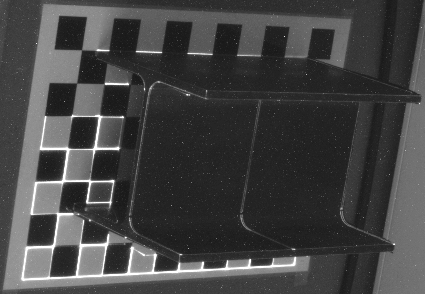
\includegraphics[height=.25\textheight]{preliminary-work/laser-beam-outline-with-chessboard-and-welding}}
		{\caption{Projection of beam outline, middle welding place and validation pattern}\label{fig:laser-beam-outline-with-chessboard-and-welding}}
		\ffigbox[\FBwidth]
		{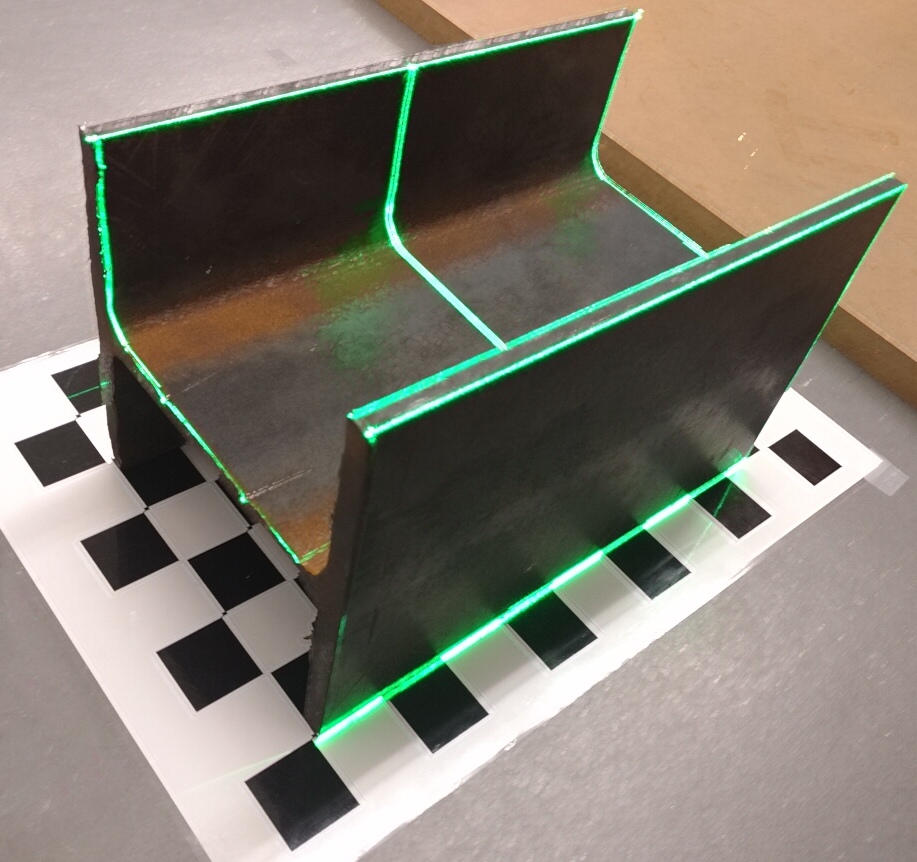
\includegraphics[height=.25\textheight]{preliminary-work/laser-beam-outline-with-welding}}
		{\caption{Projection of beam outline and middle welding place}\label{fig:laser-beam-outline-with-welding}}
	\end{floatrow}
\end{figure}

\begin{figure}[H]
	\begin{floatrow}[2]
		\ffigbox[\FBwidth]
		{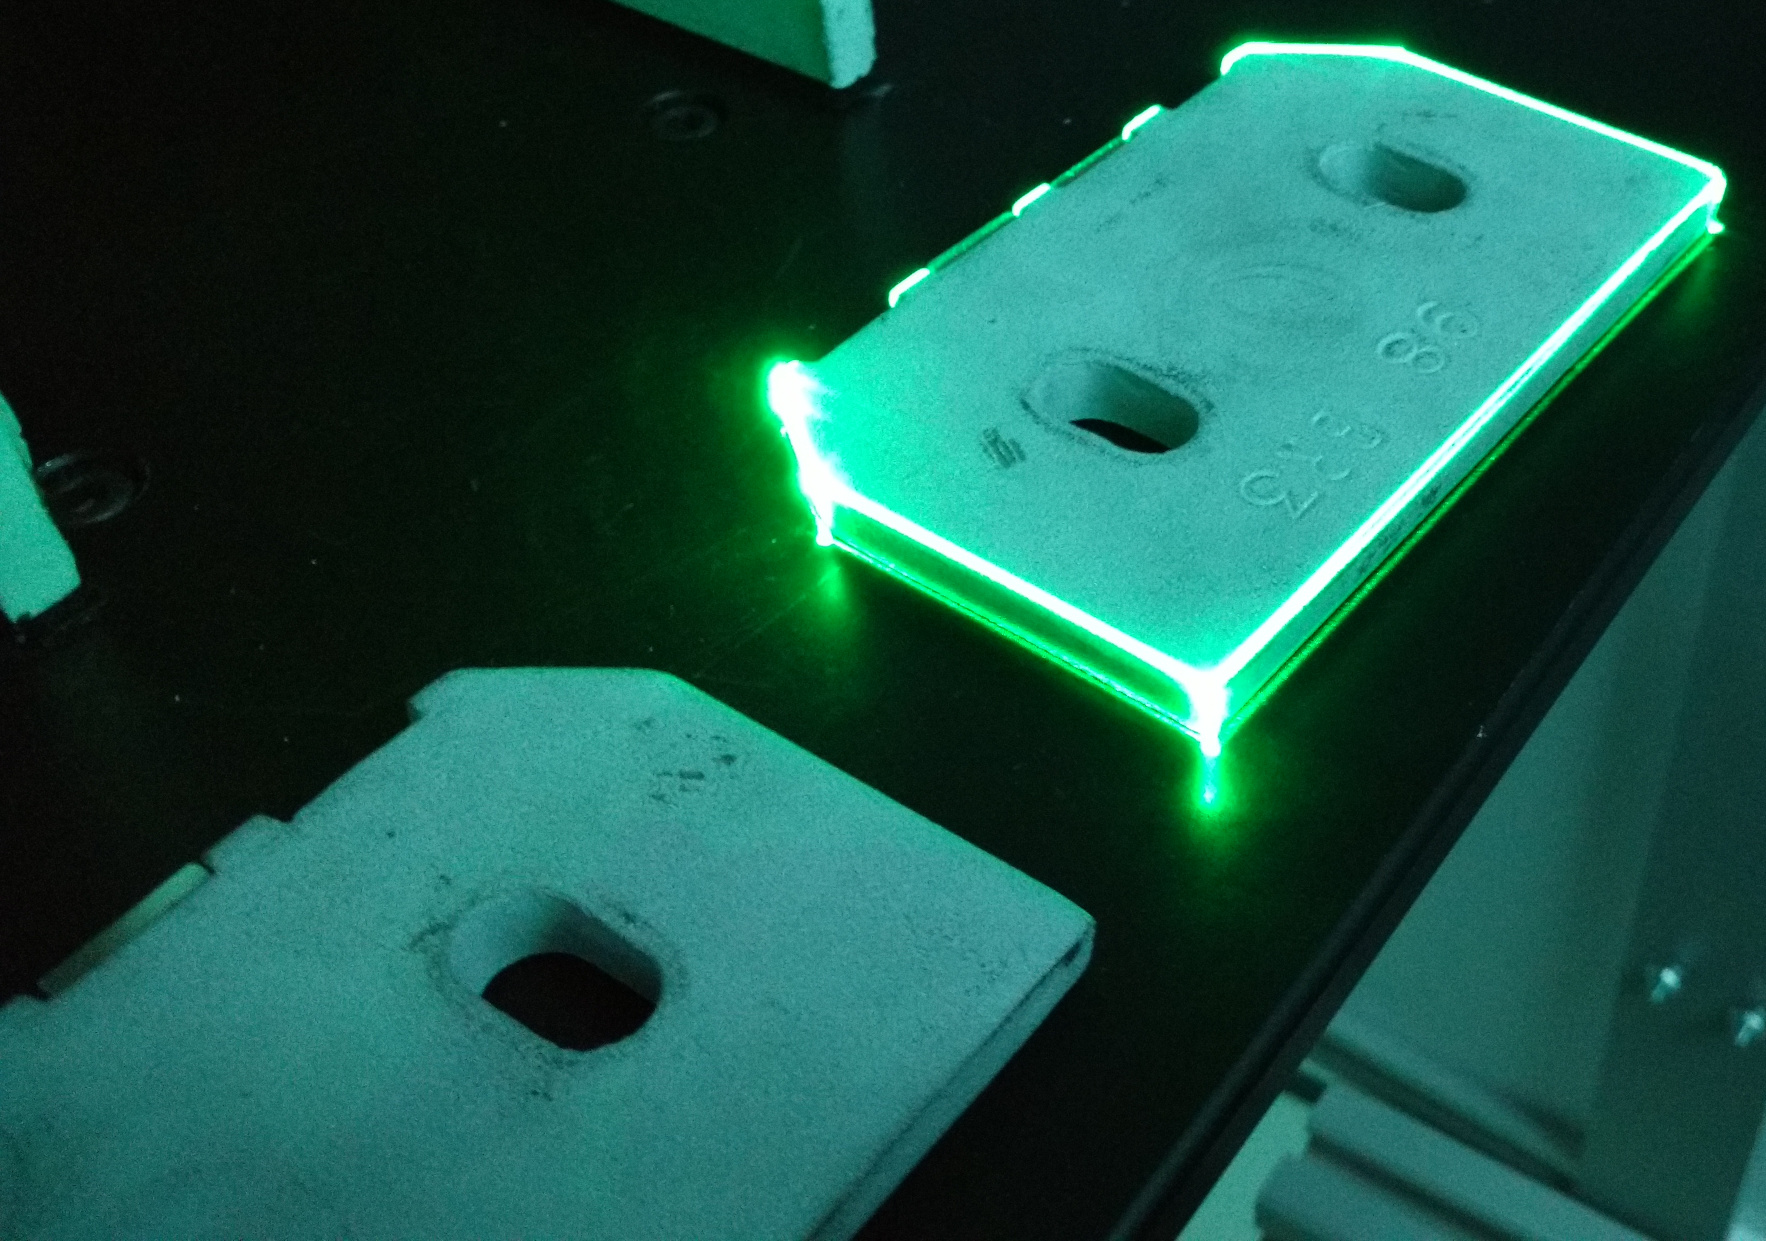
\includegraphics[height=.22\textheight]{preliminary-work/laser-object-outline}}
		{\caption{Projection of welding object outline}\label{fig:laser-object-outline}}
		\ffigbox[\FBwidth]
		{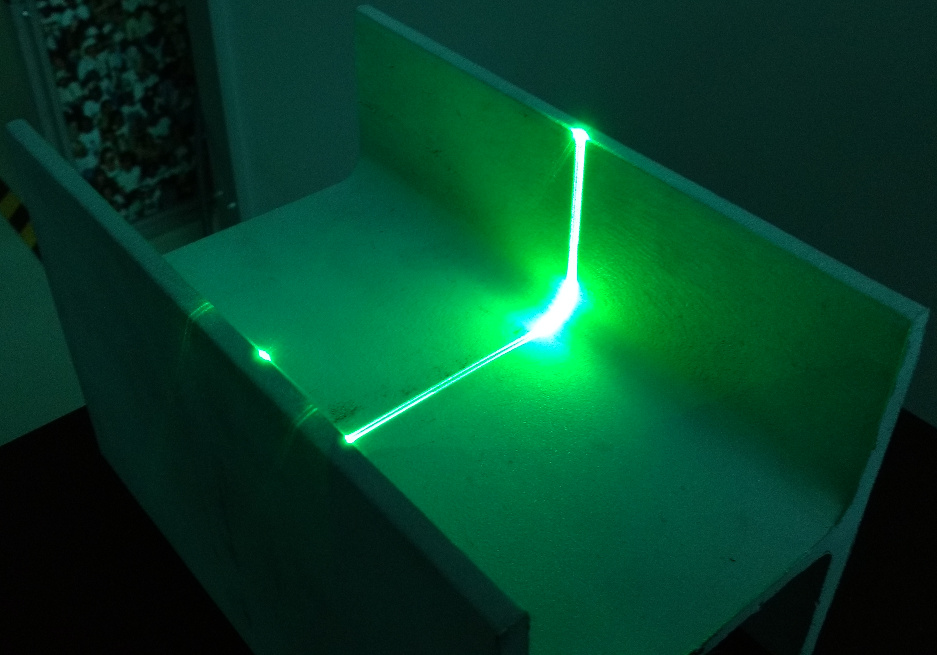
\includegraphics[height=.22\textheight]{preliminary-work/laser-welding-place}}
		{\caption{Projection of welding place in middle of beam}\label{fig:laser-welding-place}}
	\end{floatrow}
\end{figure}
